\section{Introduction}

\begin{wrapfigure}{r}{0.45\textwidth}
\vspace{-6mm}
	\centering
	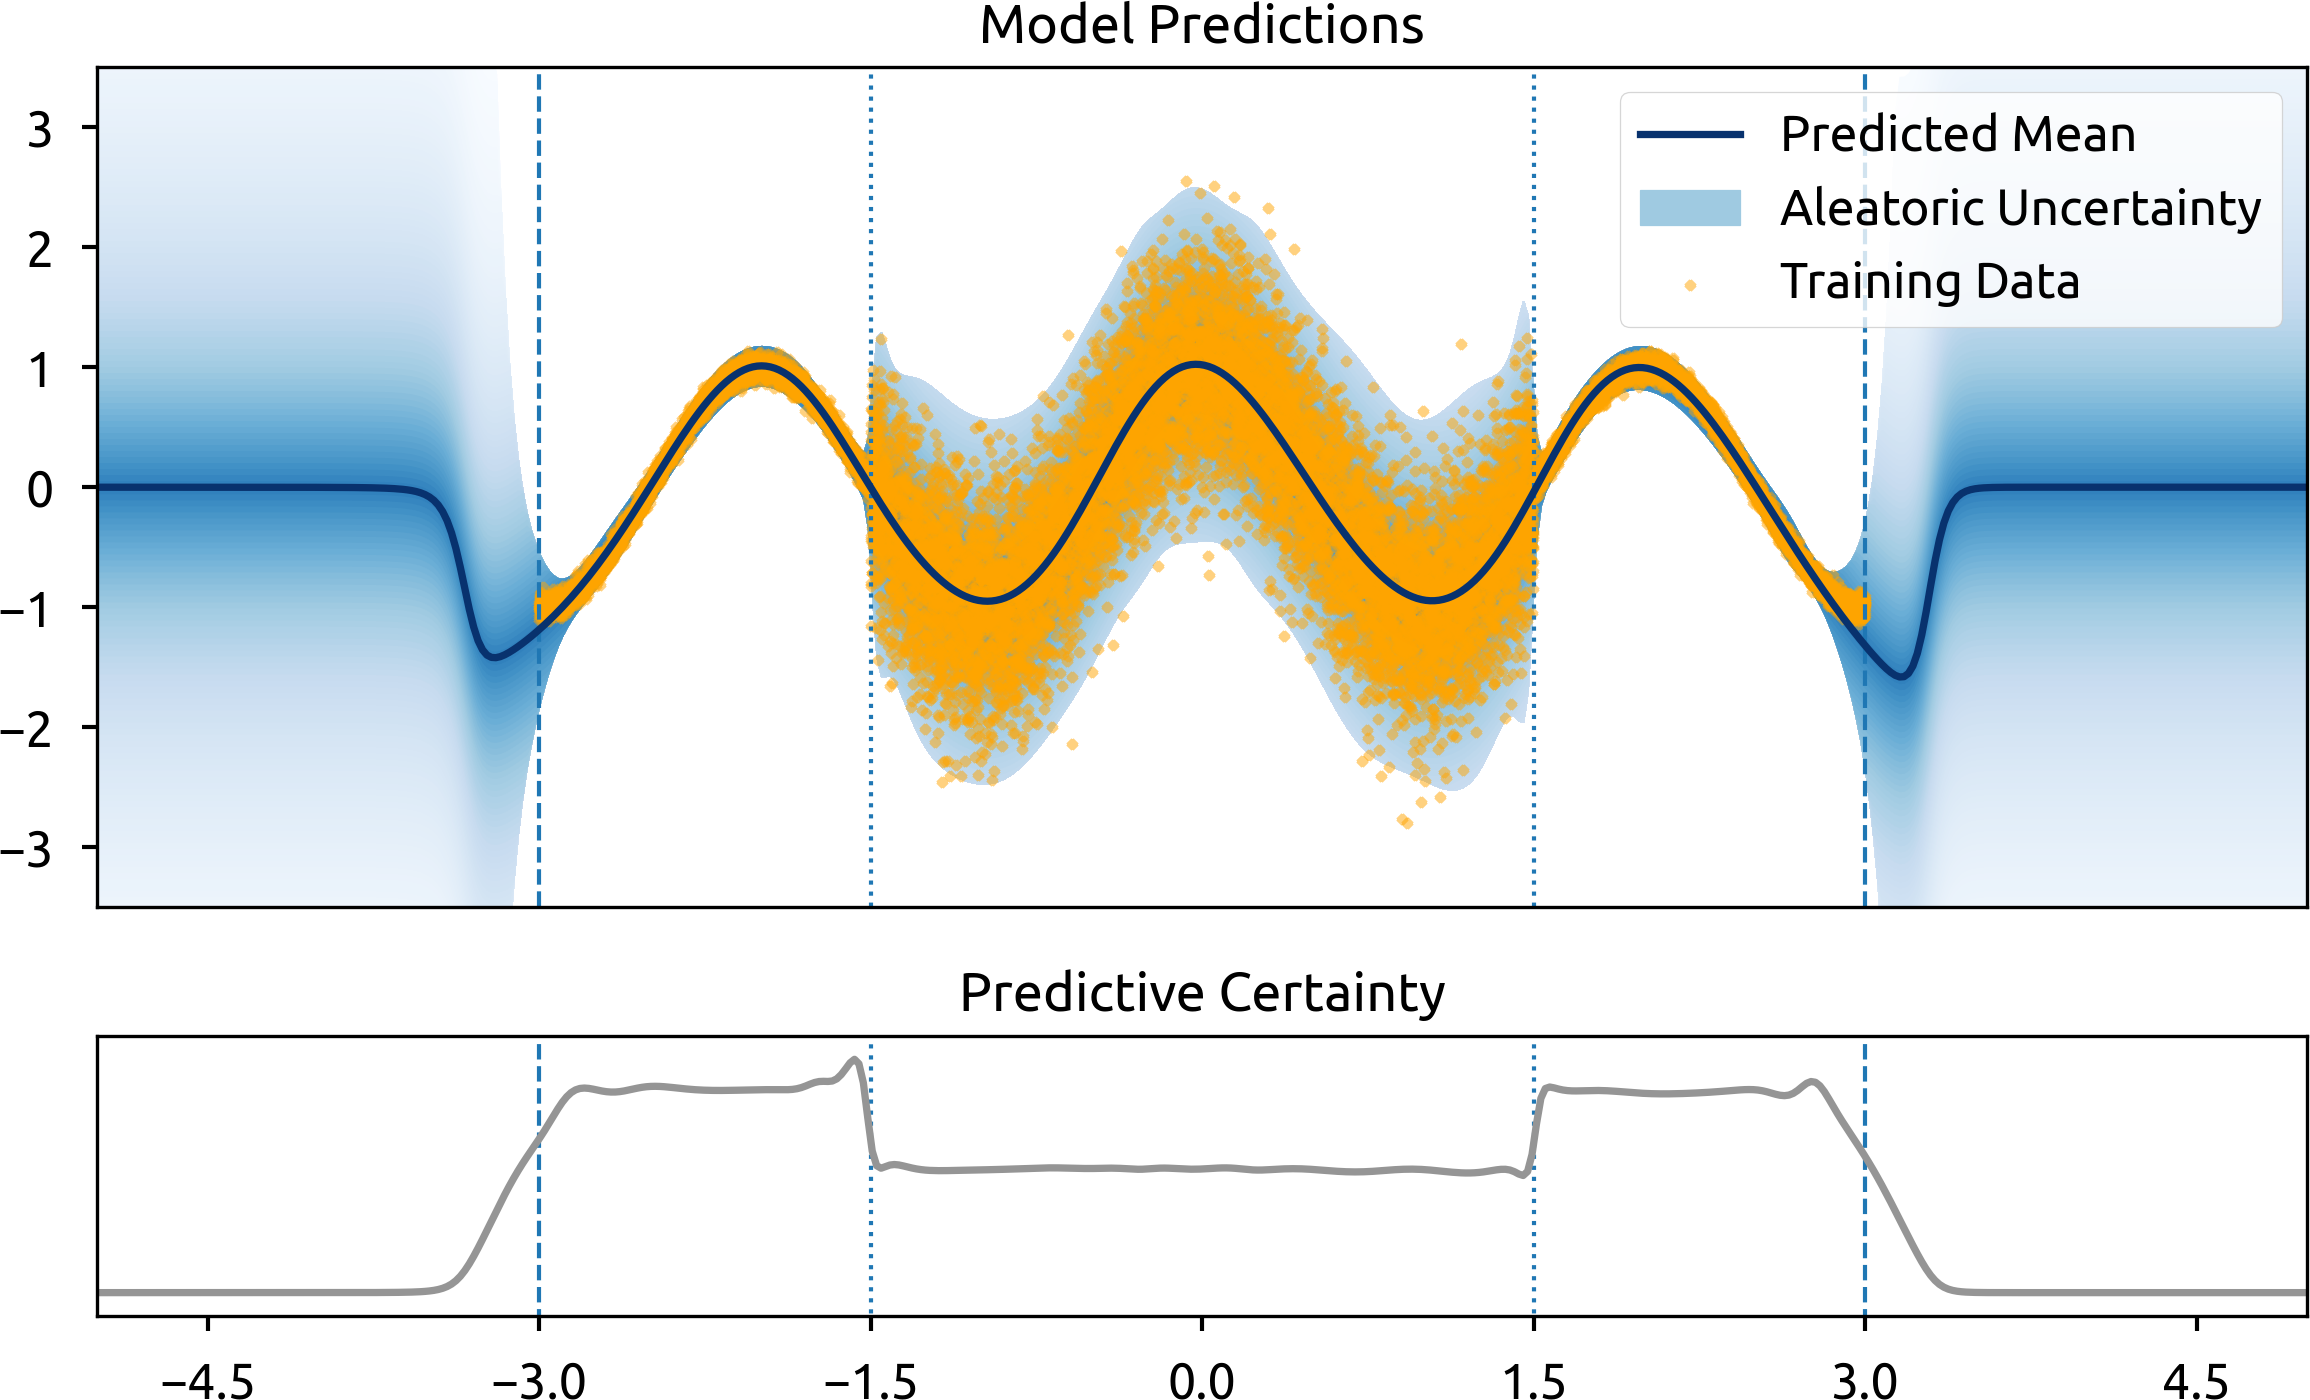
\includegraphics[width=0.42\textwidth]{sections/007_iclr2022/resources/toy-regression-trimmed.png}
    \caption*{Toy Regression Task}
    \vspace{0.3cm}
    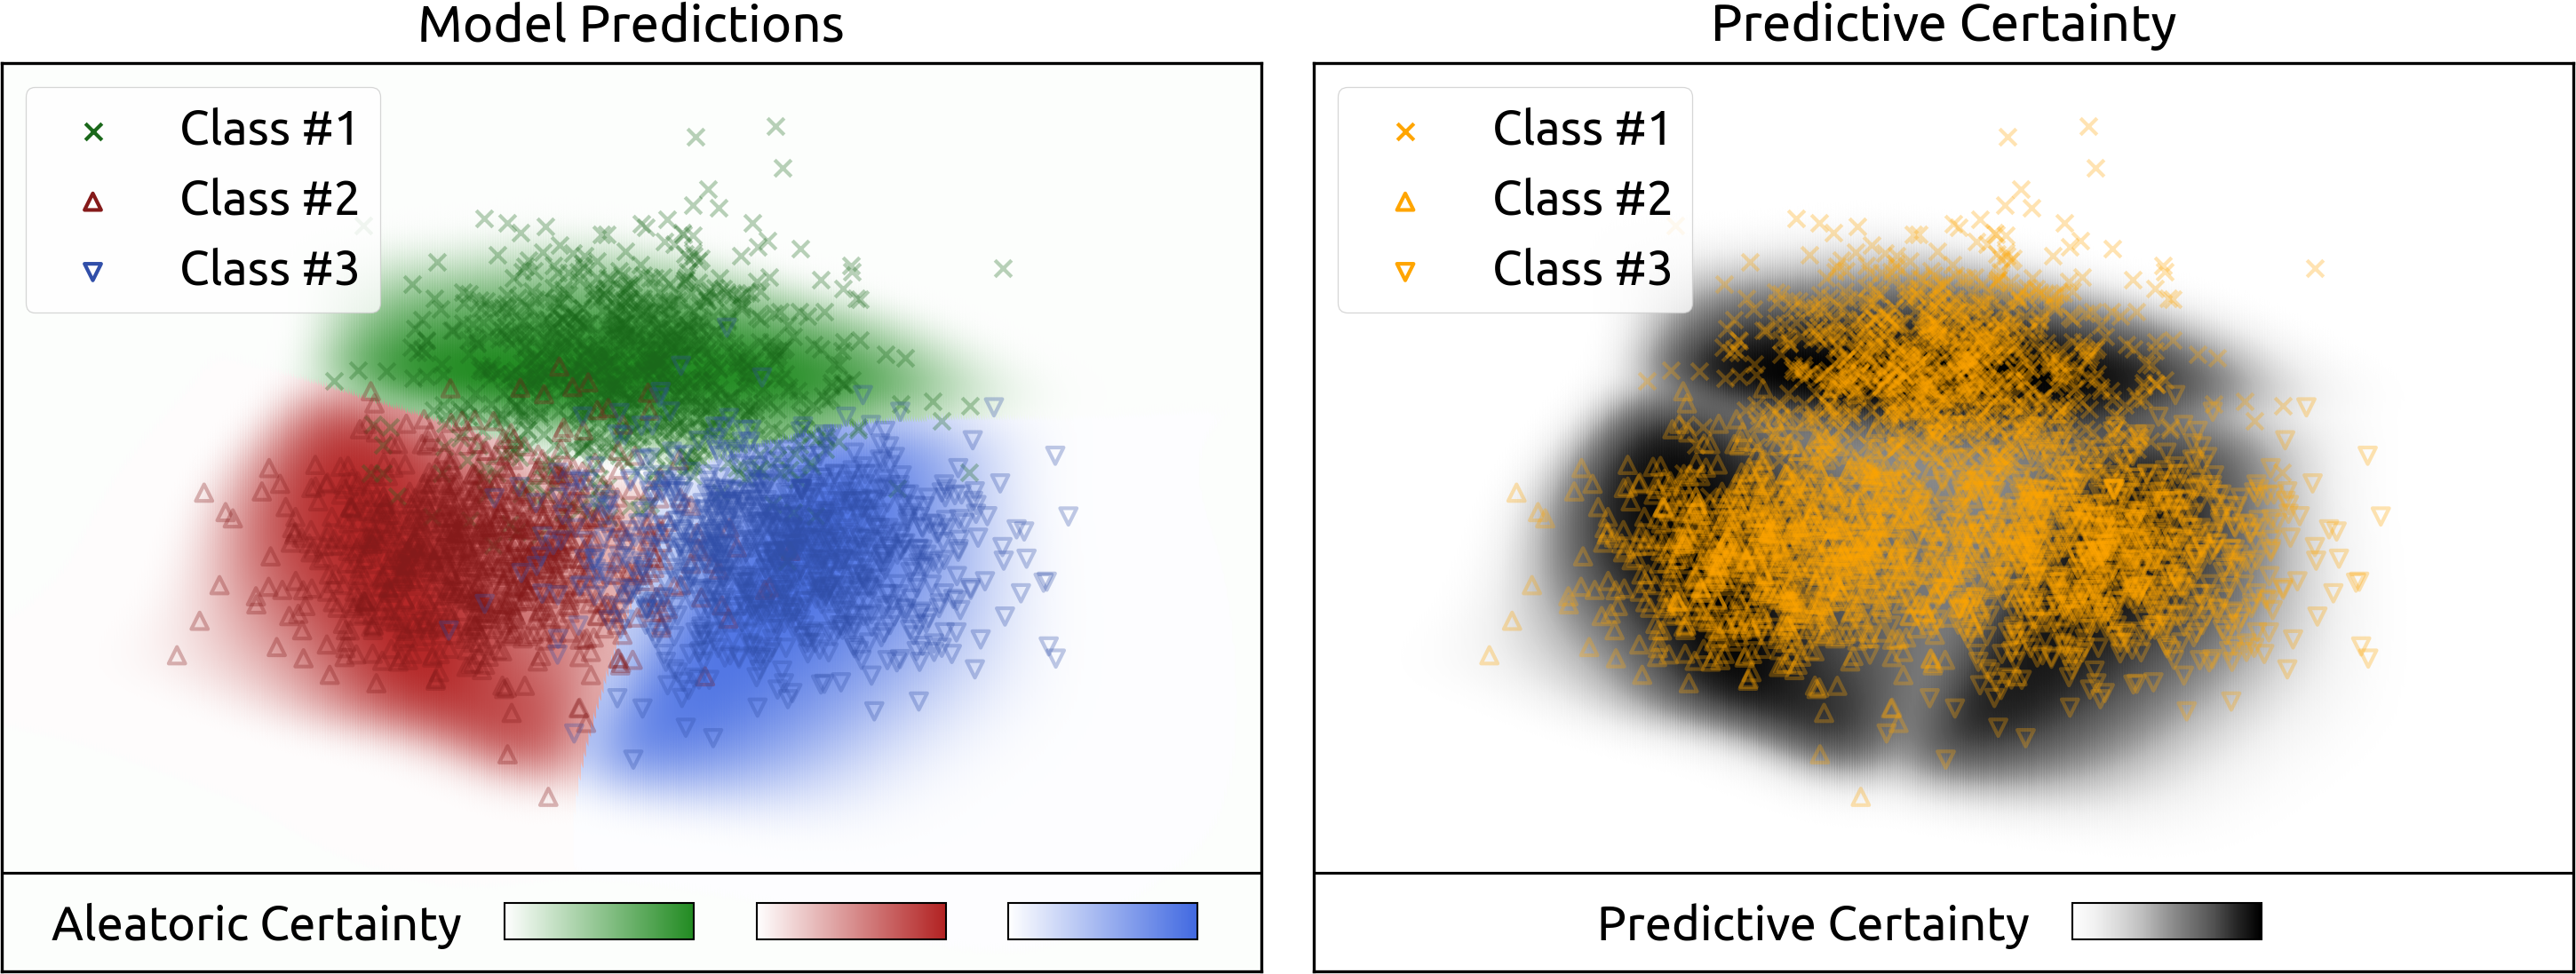
\includegraphics[width=0.42\textwidth]{sections/007_iclr2022/resources/toy-classification-trimmed.png}
    \caption*{Toy Classification Task}
    \caption{Visualization of the aleatoric and predictive uncertainty estimates of \NatPNacro{} on two toy regressions and classification tasks. \NatPNacro{} correctly assigns higher uncertainty to regions far from the training data.}
    \label{fig:toy-example-uncertainty}
    \vspace{-6mm}
\end{wrapfigure}

Accurate and rigorous uncertainty estimation is key for reliable machine learning models in safety-critical domains. It quantifies the confidence of machine learning models, thus allowing them to validate knowledgeable predictions corresponding to correct/wrong predictions, flag predictions on unknown input domains corresponding to anomaly or Out-of-Distribution detection, or detect natural shifts of the data facilitating real-time model maintenance \citep{dataset-shift, shifts-dataset, comparison-bayesian-diabetic}. Specifically, a reliable model can handle all these failure modes with high-quality estimates of \emph{aleatoric} and \emph{epistemic} uncertainty \citep{uncertainty-deep-learning}. These two levels of uncertainty allow a model to account for both irreducible data uncertainty (e.g. a fair dice's chance of $1/6$ for each face) and uncertainty due to the lack of knowledge about unseen data (e.g. input features differing significantly from training data or a covariate shift) respectively. Aleatoric and epistemic uncertainty levels can eventually be combined into an overall \emph{predictive uncertainty} \citep{uncertainty-deep-learning}

Traditional neural networks are not readily applicable in safety-critical domains as they show overconfident prediction, in particular on data that is different from training data \citep{calibration-network, ensembles}. To mitigate this problem, an important model family for uncertainty estimation directly predicts the parameters of a \emph{conjugate prior distribution} on the predicted \emph{target probability distribution}, thus accounting for the different levels of uncertainty. These models are efficient as they only require \emph{a single forward pass} for target and uncertainty prediction. Most of those models focus on classification and thus predict parameters of a Dirichlet distribution \citep{uceloss,postnet,priornet,reverse-kl,max_gap_id_ood,uncertainty-generative-classifier,multifaceted_uncertainty,graph_posterior,graph_uncertainty, lightweight-prob-net}. However, only two works \citep{evidential-regression, regression-priornet} have focused on regression by learning parameters of a Normal Inverse-Gamma (NIG) distribution as conjugate prior. Hence, all these models are limited to a \emph{single} task (e.g. either classification or regression). Some approaches even require out-of-distribution (OOD) data at training time \citep{priornet, reverse-kl} which is an unrealistic assumption in many real-world applications where anomalies are a priori diverse, rare or unknown.

\textbf{Our contribution.} We propose \NatPN{} (\NatPNacro{}) as a new approach parametrizing conjugate prior distributions for versatile uncertainty estimation. \NatPNacro{}{} is motivated from both the theoretical and practical perspective. 
\textbf{(1)} \NatPNacro{} can estimate predictive uncertainty for \emph{any} task described by the general group of exponential family distributions contrary to existing approaches from this family of models. Notably, this encompasses very common tasks such as classification, regression and count prediction which can be described with Categorical, Normal and Poisson distributions, respectively. 
\textbf{(2)} In theory, \NatPNacro{} is based on a \emph{new unified exponential family framework} which performs an input-dependent Bayesian update. For every input, it predicts the parameters of the posterior over the target exponential family distribution. We show that this Bayesian update is \emph{guaranteed} to predict high uncertainty far from training data.
\textbf{(3)} In practice, \NatPNacro{} requires \emph{no OOD data for training}, only adds \emph{a single normalizing flow} density to the last predictor layer and provides fast uncertainty estimation in a \emph{single forward pass}. Our extensive experiments showcase the high performances of \NatPNacro{} for various criteria (accuracy, calibration, OOD and shift detection) and tasks (classification, regression and count prediction). We illustrate the accurate aleatoric and predictive uncertainty predictions of \NatPNacro{} on two toy examples for classification and regression in Fig.~\ref{fig:toy-example-uncertainty}. \emph{None of the conjugate prior related works} have similar theoretical and practical properties.

%flexible, sound, simple, high quality, fast
